%%%%%%   TIPO DE DOCUMEN%TO: Reporte   %%%%%%
\documentclass[letterpaper,11pt]{report}
%%%%%%%%%%%%%%%%%%%%%%%%%%%%%%%%%%%%%%%%%%%%

%%%%%%%   PAQUETES   %%%%%%%
%\usepackage[spanish]{babel}
\usepackage{graphicx}
\usepackage{indentfirst}
\usepackage[utf8]{inputenc}
\usepackage [margin=1in,includefoot]{geometry}
\usepackage{colortbl}
\usepackage{array,booktabs,xcolor}  %arydshln,multirow
\usepackage{caption}
\usepackage{multirow}
\usepackage{enumerate}
\newcommand\VRule[1][\arrayrulewidth]{\vrule width #1}
%%%%%%%%%%%%%%%%%%%%%%%%%%%%

%%%%%%%%%%%%%%%%%%%%%%%%%%%%%%%%%%%%%%%%
%%%%%%%   INICIO DEL DOCUMENTO   %%%%%%%
%%%%%%%%%%%%%%%%%%%%%%%%%%%%%%%%%%%%%%%%
\begin{document}

    %%%%%%% Renombrar en espaNol %%%%%%
    \renewcommand\bibname{Bibliografía}
    \renewcommand{\figurename}{Figura}
    \renewcommand{\tablename}{Tabla} %Escribe Tabla en lugar de Cuadro
    \renewcommand{\listtablename}{\'Indice de tablas} %Escribe Indeice de tablas en lugar de Indice de cuadros
    \renewcommand{\chaptername}{Capítulo}
    \renewcommand*{\contentsname}{Contenido}
    \renewcommand\listfigurename{Lista de figuras}

    %%%%%%%   PORTADA   y RESUMEN   %%%%%%% Este es el contenido agregado de la secci\'on 2.

    %%%%%%%%%%%%%%%%%%%%%%%%%%%%%
%%%%%      PORTADA      %%%%%
%%%%%%%%%%%%%%%%%%%%%%%%%%%%%

\begin{titlepage}

    \centering %Todo centrado

    %%%%  LOGO DE LA ESCUELA   %%%%
    
\includegraphics[scale=0.17]{imagenes/escom-ipn} %Imagen para portada
    %%%%  NOMBRE DE LA ESCUELA   %%%%
    \LARGE{\\ Instituto Polit\'ecnico Nacional}
    \LARGE{\\ Escuela Superior de C\'omputo}
    
    \vspace{1cm} %Espacio vertical

    %%%%  TITULO Y NÚMERO DE TRABAJO   %%%%
    \LARGE \textbf{Augmented Reality Furniture (ARF)}
    \LARGE {\\ TT2018-A002}

    \vspace{1cm} %Espacio vertical

    \LARGE \textit{Que para cumplir con la opción de titulación curricular en la carrera de:}
    \LARGE \textbf{\\ Ingeniería en Sistemas Computacionales}

    \vspace{1cm} %Espacio vertical

    %%%%   ALUMNOS   %%%%
   \textit{Presentan}\\
    Cabello Acosta Gerardo Aramis\\
    Carrillo Mendoza Martín Alejandro \\
    Del Pilar Morales Saúl

    \vspace{1cm} %Espacio vertical

    %%%%   Directores   %%%%
   \textit{Directores}\\
    M. en C. Vélez Saldaña Ulises. \bigskip  \\
    M. en C. José David Ortega Pacheco. \bigskip  
\end{titlepage} %incluye el archivo portada.tex
    %%%%%%%%%%%%%%%%%%%%%%%
%%%%    RESUMEN    %%%%
%%%%%%%%%%%%%%%%%%%%%%%

\begin{abstract}

  Aquí va el resumen general del documento de trabajo terminal.

\end{abstract}
 %Incluir resumen del documento (resumen.tex)

    %%%%%%%   INCLUIR ENCABEZADOS EN INDICES Y CAPITULOS   %%%%%%%
    \pagestyle{headings}

    %%%%%%%   NUMERACION EN CONTENIDO E INDICE DE TABLAS Y FIGURAS   %%%%%%%
    \pagenumbering{roman} %NUmeros romanos
    %\setcounter{page}{1} %Comienza en I por default, aquI se puedo modificar

    %%%%%%   INCLUIR CONTENIDO, INDICE DE FIGURAS E INDICE DE TABLAS   %%%%%%
    \tableofcontents
    \listoffigures
    \listoftables

    %%%%%%%   NUMERACION EN CAPITULOS   %%%%%%%
    \clearpage %Para iniciar con los arAbigos
    \pagenumbering{arabic} %Numeros arabigos
    %\setcounter{page}{1} %Comienza en 1 por default, aquI se puede modificar

    %%%%%%%   INCLUYE CAPITULOS Y SECCIONES   %%%%%%%
    \chapter{Introducci\'on}

En éste capítulo se define el contexto del trabajo terminal, el problema que vamos a abordar y por qué lo vamos a resolver, cuáles son nuestros objetivos y cómo vamos a lograr solucionar el problema planteado. También está descrito el trabajo previo (estado del arte) el cual aborda la problemática que escogimos
	   \section{Contexto de trabajo}

Actualmente vivimos en un entorno dominado por la tecnología; día a día se desarrollan nuevas herramientas con el fin de ayudar al ser humano a realizar tareas de una forma más fácil y eficiente, como los HMD (Head-mounted Display)\cite{B15}.


Por otro lado también nos encontramos en una época donde el diseño es un área de gran importancia en cualquier sector del mercado, por ejemplo, un buen diseño web en un sitio es fundamental lograr que un producto se logre vender o difundir, un buen diseño gráfico en campañas de marketing asegura más clientes; de igual forma nos encontramos con el diseño de interiores. Para esta última área se suelen contratar diseñadores de interiores profesionales para lograr que los espacios interiores de un inmueble consigan tal armonía que mejoren la calidad de vida de quienes lo habitan y además generen un impacto en las personas que usan éstas habitaciones.\par
El diseño de interiores profesional no sigue un proceso estandarizado, sin embargo a nivel general podemos ubicar las siguientes etapas:

\begin{itemize}
	\item El cliente acude con un diseñador de interiores profesional, quien acude al domicilio para conocer las condiciones del inmueble y conocer las necesidades y presupuesto del cliente.
	\item Conociendo estos dos puntos el diseñador hace un análisis de viabilidad que se compone de un análisis presupuestal y la definición del alcance del diseño.
	\item El diseñador le muestra esta información al cliente para que la apruebe, en caso de no ser así, el proyecto es considerado como no viable.
	\item De ser viable el diseñador de interiores genera un calendario previo de actividades donde programa el cumplimiento de los requerimientos del cliente en determinadas fechas.
	\item Si el cliente aprueba la propuesta de calendario, el diseñador se dispone a realizar el \textbf{proceso de propuesta de diseño de interiores} con el objetivo de mostrarle al cliente el resultado final previo de la obra antes de que sea realizada, esta propuesta puede mostrarse de varias formas como fotografías con fotomontajes, una explicación verbal con fotografías de apoyo (de muebles o habitaciones ya decoradas) o un modelado tridimensional del resultado de la obra; se suele usar un modelado tridimensional pues es lo más cercano a la realidad que se le puede mostrar al cliente. Si el cliente no aprueba la propuesta de calendario, se debe volver a realizar el análisis de viabilidad para ajustarse a las necesidades y presupuesto del cliente.
	\item El diseñador le muestra la propuesta de diseño al cliente y si esta es aceptada, se inicia el desarrollo de la obra con base en las fechas establecidas.
	\item Finalmente el diseñador entrega la obra al cliente y termina el proceso de diseño de interiores.
\end{itemize}

El proceso completo anteriormente descrito se puede observar en la figura 1.1 a través de un diagrama de proceso de negocio, en las figuras 1.2 y 1.3 se muestra el diagrama segmentado para una mejor lectura del mismo, y en la figura 1.4 puede observar el \textbf{proceso de propuesta de diseño de interiores}.\par
Teniendo a la mano una gran diversidad de herramientas tecnológicas, podemos usar estos elementos para lograr que el diseño de interiores sea más sencillo y rápido, tanto para un diseñador de interiores que vaya a realizar una obra para algún cliente, como para alguien que desee diseñar o rediseñar su propio inmueble.
\newpage

\begin{figure}[!htbp]
	\centering
	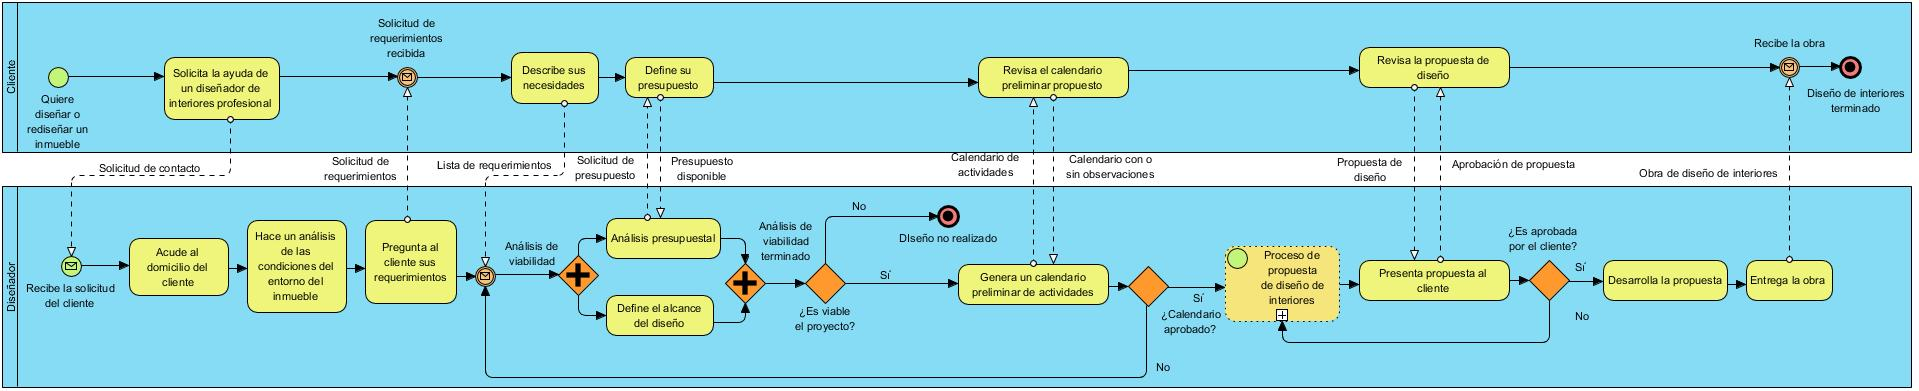
\includegraphics[width=20cm,angle=270,origin=c]{imagenes/marcoteorico/bpmn/proceso_full.jpg}
	\caption{Modelo del proceso de diseño de interiores (Completo).}
	\label{fig:bpmn_antes}
\end{figure}
\newpage

\begin{figure}[!htbp]
	\centering
	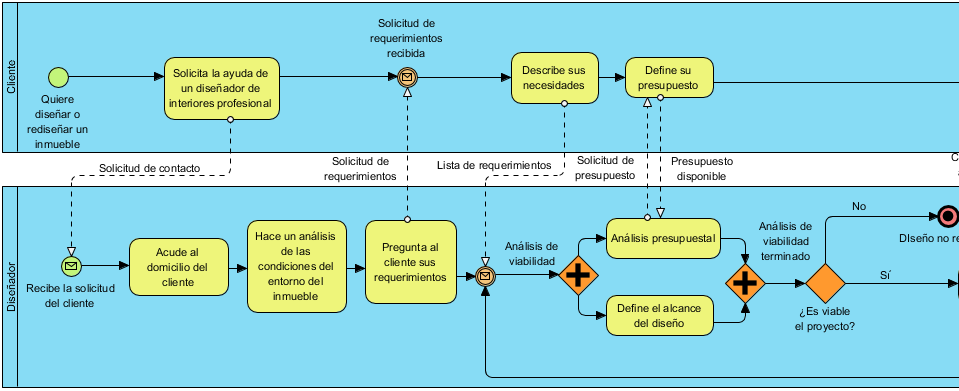
\includegraphics[width=19cm,angle=270,origin=c]{imagenes/marcoteorico/bpmn/proceso_01_01_left.png}
	\caption{Modelo del proceso de diseño de interiores (Segmento I).}
	\label{fig:bpmn_antes}
\end{figure}
\newpage

\begin{figure}[!htbp]
	\centering
	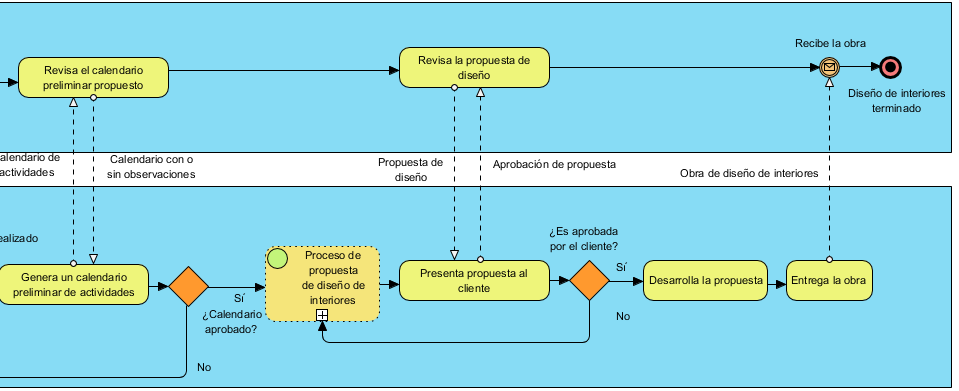
\includegraphics[width=19cm,angle=270,origin=c]{imagenes/marcoteorico/bpmn/proceso_02_01_left.png}
	\caption{Modelo del proceso de diseño de interiores (Segmento II).}
	\label{fig:bpmn_antes}
\end{figure}
\newpage

\begin{figure}[!htbp]
	\centering
	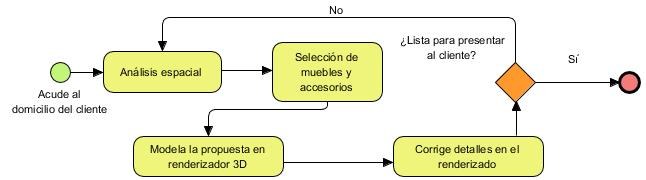
\includegraphics[width=16cm]{imagenes/marcoteorico/bpmn/subproceso.jpg}
	\caption{Subproceso de propuesta de diseño de interiores.}
	\label{fig:subproceso}
\end{figure}
\newpage
	   \section{Problemática}
El diseño de interiores para las personas en general, es un proceso complejo, tardado y tedioso, debido a la implicación del tratamiento superficial y el manejo del volúmen espacial, lo cual puede provocar pérdidas económicas y de tiempo por parte del cliente que compra un mueble y/o por parte de la tienda si se efectúa un proceso de devolución de producto dañando el prestigio de la tienda o sucursal asociada a la venta de estos muebles u objetos.

   
	   \section{Trabajo previo}
Las aplicaciones y proyectos que abordan el problema anteriormente descrito son:

\begin{enumerate}
	\item Canvas (iOS).
	\item Amazon App.
	\item Fingo.
	\item Ikea Place.
	\item TT 2012-B043. Realidad aumentada aplicada a la decoración de interiores.
\end{enumerate}

De forma colectiva, en tales aplicaciones pudimos notar las siguientes características:

\begin{enumerate}
	\item La cámara puede escanear una habitación para conocer los planos donde puede posicionar muebles.
	\item El usuario puede exportar el escaneo tridimensional de una habitación para usarlo en AutoCAD.
	\item Mediante realidad aumentada el usuario puede posicionar un objeto a donde enfoque la cámara del celular.
	\item Existe una posición relativa de los objetos, es decir, si el celular se mueve el objeto permanece en la misma posición.
	\item Se requiere un hardware especial además del dispositivo móvil.
\end{enumerate}

Cabe destacar que Fingo y el TT 2012-B043 utilizan marcadores físicos, colocados en el suelo, sobre los cuales se superponen los objetos tridimensionales, lo cual limita su uso, dado que son dependientes de un elemento externo.\par
Por otro lado, encontramos características que consideramos importantes para resolver el problema planteado, pero ninguna de las aplicaciones anteriores las posee, como son:


\begin{enumerate}
	%\item No están enfocadas a e-Commerce
	\item No existe un gran repertorio de submodelos de objetos
	\item No poseen valores agregados en los objetos en general, por ejemplo, que se muestre el costo de un producto.
	\item No muestra presupuestos generales que indiquen los costos de los productos agregados al entorno de realidad aumentada, ni permite definir un presupuesto inicial que limite los objetos que se van a agregar.
	\item No permiten guardar información relacionada a los entornos de realidad aumentada generados.
\end{enumerate}

En la \textbf{\textit{Tabla 1.1}} podemos apreciar una comparación de las aplicaciones anteriores y la aplicación que planeamos hacer con base en las características previamente descritas:\par

% Please add the following required packages to your document preamble:
% \usepackage{graphicx}
% \usepackage[table,xcdraw]{xcolor}
% If you use beamer only pass "xcolor=table" option, i.e. \documentclass[xcolor=table]{beamer}
\begin{table}[!hbtp]
	\resizebox{\textwidth}{!}{%
		\begin{tabular}{|l|l|l|l|l|l|l|}
			\hline
			\textbf{Características}       & \textbf{Canvas}                                 & \textbf{Tango}           & \textbf{Fingo}           & \textbf{Ikea Place}      & \textbf{TT 2012-B043}    & \textbf{Nuestra App}     \\ \hline
			Escaneo                        & \cellcolor[HTML]{BFBFBF}{\color[HTML]{C0C0C0} } &                          & \cellcolor[HTML]{BFBFBF} & \cellcolor[HTML]{FFFFFF} & \cellcolor[HTML]{BFBFBF} & \cellcolor[HTML]{BFBFBF} \\ \hline
			Exportar                       & \cellcolor[HTML]{BFBFBF}                        &                          &                          & \cellcolor[HTML]{FFFFFF} & \cellcolor[HTML]{FFFFFF} &                          \\ \hline
			Enfoque                        &                                                 & \cellcolor[HTML]{BFBFBF} &                          & \cellcolor[HTML]{BFBFBF} & \cellcolor[HTML]{BFBFBF} & \cellcolor[HTML]{BFBFBF} \\ \hline
			Posición relativa              &                                                 & \cellcolor[HTML]{BFBFBF} &                          & \cellcolor[HTML]{BFBFBF} & \cellcolor[HTML]{FFFFFF} & \cellcolor[HTML]{BFBFBF} \\ \hline
			Hardware externo               & \cellcolor[HTML]{BFBFBF}                        &                          & \cellcolor[HTML]{BFBFBF} & \cellcolor[HTML]{BFBFBF} & \cellcolor[HTML]{BFBFBF} &                          \\ \hline
			Variedad                       &                                                 &                          & \cellcolor[HTML]{BFBFBF} & \cellcolor[HTML]{FFFFFF} & \cellcolor[HTML]{BFBFBF} & \cellcolor[HTML]{BFBFBF} \\ \hline
			Diseños realistas de objetos   &                                                 &                          & \cellcolor[HTML]{BFBFBF} & \cellcolor[HTML]{BFBFBF} & \cellcolor[HTML]{FFFFFF} & \cellcolor[HTML]{BFBFBF} \\ \hline
			Valor agregado                 &                                                 &                          & \cellcolor[HTML]{BFBFBF} & \cellcolor[HTML]{BFBFBF} & \cellcolor[HTML]{FFFFFF} & \cellcolor[HTML]{BFBFBF} \\ \hline
			Presupuesto general            &                                                 &                          &                          &                          &                          & \cellcolor[HTML]{BFBFBF} \\ \hline
			Presupuesto inicial            &                                                 &                          &                          &                          &                          & \cellcolor[HTML]{BFBFBF} \\ \hline
			Guardar información del diseño &                                                 &                          &                          &                          &                          & \cellcolor[HTML]{BFBFBF} \\ \hline
		\end{tabular}%
	}
	\caption{Comparativo de aplicaciones sobre diseño de interiores}
	\label{comparativoestadodelarte}
\end{table}
	   \section{Solución propuesta}
Para mejorar el proceso de diseño de interiores, proponemos desarrollar una aplicación móvil que permita a los usuarios visualizar a través de la realidad aumentada muebles y objetos decorativos en una habitación, eliminando la necesidad de tenerlos físicamente en ella, la cual servirá como herramienta de apoyo en este proceso; así se reducirá el número de etapas del proceso de diseño de interiores volviéndolo más sencillo y rápido.

 
	   \section{Objetivo}
\subsection{Objetivo general}
Desarrollar una aplicación móvil que permita crear entornos virtuales utilizando realidad aumentada en dispositivos móviles para facilitar y agilizar el proceso de diseño de interiores.

\subsection{Objetivos específicos}
\begin{itemize}
	\item Implementar una forma de visualización de muebles utilizando la realidad aumentada.
	\item Desarrollar una nueva propuesta de diseño de interiores para que los diseñadores de interiores puedan presentar a sus clientes.
	\item Poder almacenar las propuestas de diseño de interiores generadas.
	\item Desarrollar una forma para poder presentar análisis presupuestales de diseños de interiores.
	\item Poder agrupar las propuestas de diseño de interiores por cliente y almacenar información del mismo.
	\item Poder ajustar el costo final de los escenarios creados a través de la definición inicial del presupuesto del cliente.
\end{itemize}
	   \section{Justificación}


    \chapter{Marco Teórico }
	El presente trabajo pretende analizar y documentar el desarrollo de una aplicación móvil para el diseño de interiores, por ello las definiciones que a continuación se exponen son necesarias para entender objetivo y el funcionamiento del software.
	
	   \section{Diseño de interiores}
\subsection{Definicion}
El diseño de interiores es una profesión en la cual soluciones creativas y técnicas son aplicadas dentro de una estructura para lograr la construcción de un entorno interno determinado. Éstas soluciones son funcionales, mejoran la calidad de vida de los ocupantes y son aestéticamente atractivas. Los diseños deben apegarse al código y normas requeridos, y fomentar los principios de sustentabilidad ambiental definidos por el edificio o empresa. El objetivo del diseño de interiores es lograr una armonía en los espacios que habitamos y dar confort al usuario de dichos espacios\cite{B01}. \par
El diseño de interiores sigue una metodología sistemática y coordinada que incluye investigación, análisis e integración de conocimientos dentro de un proceso creativo. Dentro ésta metodología podemos ubicar distintos servicios o etapas, dependiendo de la complejidad del trabajo, en las cuales encontramos: definición de los requerimientos funcionales para los espacios de las habitaciones, planeación de espacios interiores, realización de planos de construcción, definición de especificaciones de ubicación, colores y acabados en piso, paredes, materiales, equipo, mobiliario y muebles, administración de contratos de fabricación o instalación, etc.\par
En Estados Unidos el diseño de interiores es la única rama del diseño que está sujeta a las regulaciones federales y la ley gubernamental\cite{B02}.
\subsection{Movimientos en el diseño de interiores}

\subsubsection{Feng shui}
El Feng Shui es un arte utilizado actualmente para alcanzar la armonización de las energías en las casas y los lugares de trabajo, basado en principios milenarios de la sabiduría chin\cite{B26}. Surge de la conjunción de dos ideogramas chinos que significan ``viento" y ``agua", dos conceptos que para las tradiciones de la antigüedad se relacionaban con el flujo y la circulación de la energía vital. Mediante este arte, nos es posible conocer cuál es la perfecta ubicación para edificar una casa, el lugar ideal para colocar cada uno de los muebles, así como también la forma de revertir las energías adversas que puedan afectarnos. El Feng Shui estudia la relación del hombre con la naturaleza y brinda la oportunidad de vivir de acuerdo con los principios que la rigen, y de esta manera, aprovechar esas energías que fluyen por todas partes y pueden influir en nuestro bienestar general.

\subsubsection{Deconstructivismo}
El desconstructivismo es la arquitectura que busca llegar a nuevas formas de expresión al alejarse de las restricciones estructurales y jerarquías funcionales y temáticas, enfocado 
hacia diseños a menudo no rectangulares, fantásticos y aparentemente inconexos\cite{B24}. Tal trabajo a menudo representa una aplicación de las teorías filosóficas  de Jacques Derrida en Francia, que trato de llegar a nuevas ideas en la literatura; esta filosofía se ha aplicado desde finales del siglo 20 a las estructuras arquitectónicas generalmente llamadas arquitecturas deconstructivistas. \par
La arquitectura deconstructivista surge en una exposición, titulada ``Deconstructivist architecture", que Philip Johnson y Mark Wigley organizaron en el museo de Arte Moderno (MoMa) de Nueva York en 1988.

\subsubsection{Diseño Orgánico}
Arquitectura cuyo diseño se establece de acuerdo con los procesos de la naturaleza en lugar de basarse en un diseño ya impuesto. Es una filosofía de diseño propuesta por Frank Lloyd Wright (1867-1959) a comienzos del siglo 20 y en ella afirma que un edificio (y su apariencia) deben de seguir formas que estén en armonía con su entorno natural.\cite{B24}\par  
Los materiales utilizados en el exterior deben ser acoplarse con la ubicación del edificio, relacionando así el edificio con su entorno. Por lo tanto, debe hacerse de baja altura, con techos que sobresalgan para proporcionar protección del sol en el verano y para proporcionar alguna protección contra la intemperie en invierno además se debe de hacer un máxima uso de la luz natural.

\subsection{Fundamentos del diseño de interiores}
El diseño de interiores se ve como una actividad que tiene un punto de inicio (cuando el diseñador y el cliente tienen el primer contacto) y otro al final cuando el proyecto se ha ejecutado.\par
Se debe tomar en cuenta que el diseño de interiores es maleable, es decir, que su realización no está sujeto estrictamente a una serie de reglas. En un caso se puede realizar un determinado proceso, y en otro se puede realizar otro proceso diferente. No existe una solución estandarizada para para todos los casos.\par
Lo más importante es definir el por qué estamos diseñando. Por ejemplo si se está diseñando un armario, se tiene qué saber cuál es el impulso para hacerlo. El diseñador se plantea algunas ideas sobre las funciones que tiene un armario, el uso de la madera reciclada, el del plástico o un nuevo material, y con base a eso, define el objetivo de diseñar el armario.
Otro fundamento importante es la armonía que se busca. Un espacio interior no sólo debe verse bonito, y tener colores agradables a la vista. Cada elemento que compone un espacio debe relacionarse con los demás. Un sillón en una sala de espera debe relacionarse y tener alguna conexión con la mesa de centro. Esta relación puede ser la similitud del acabado de ambos, la ubicación de uno con respecto al otro, etc.
Una habitación debe seguir un esquema de colores bien definido. Dentro de estos esquemas tenemos el monocromático, complementario y análogo, y cada uno deriva del círculo cromático.\par

\textbf{Monocromático}.- Es una selección de colores que funcionen bien juntos. Esto es trabajar con un matiz, y la variación de tintes, tonos, y sombras.
\begin{figure}[h!]
	\centering
	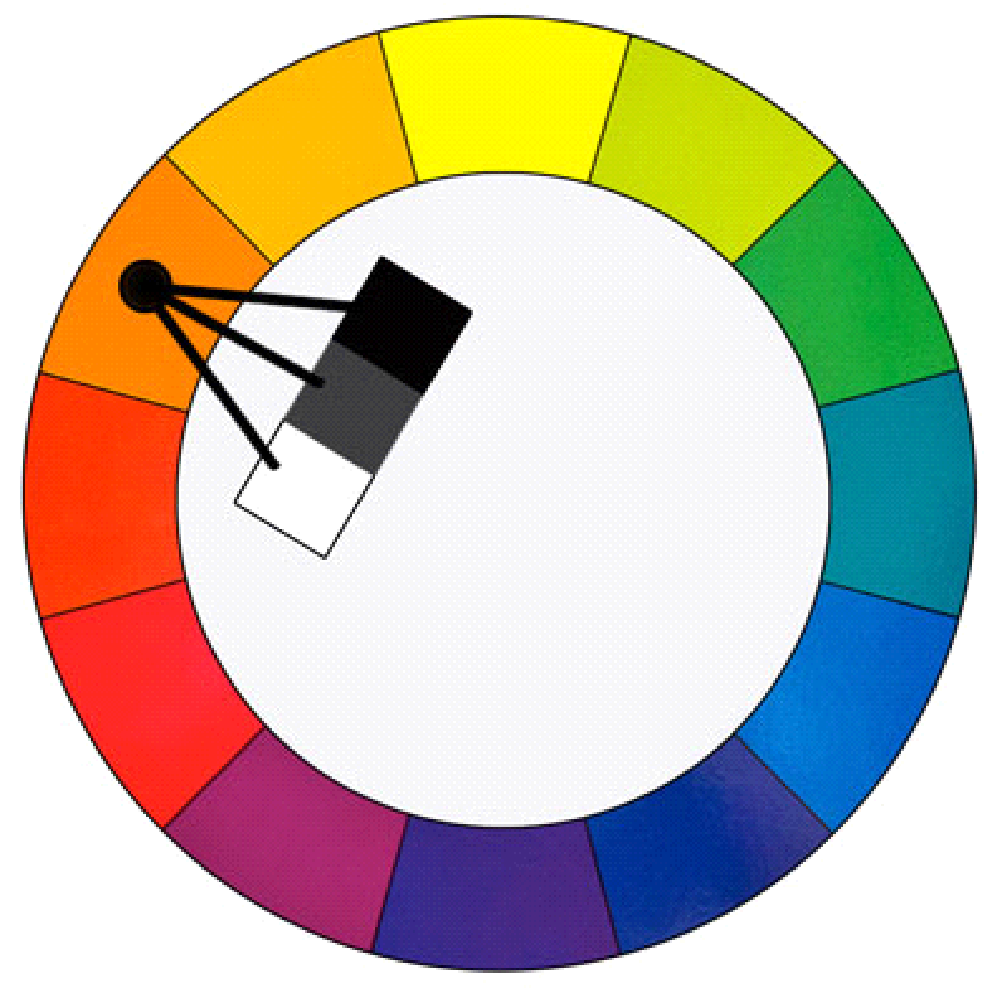
\includegraphics[width=7cm]{imagenes/marcoteorico/disenointeriores/monocromatico.png}
	\caption{Esquema monocromático.\cite{B13}}
	\label{fig:monocromatico}
\end{figure}

\textbf{Complementario}.- Los colores que se encuentran en extremos opuestos del círculo cromático se consideran complementarios. Al combinar estos dos colores, se puede expresar contraste e interés. Son difíciles de usar en grandes cantidades, pero por su contraste son muy buenos para resaltar algo, como un llamado de atención.
\begin{figure}[h!]
	\centering
	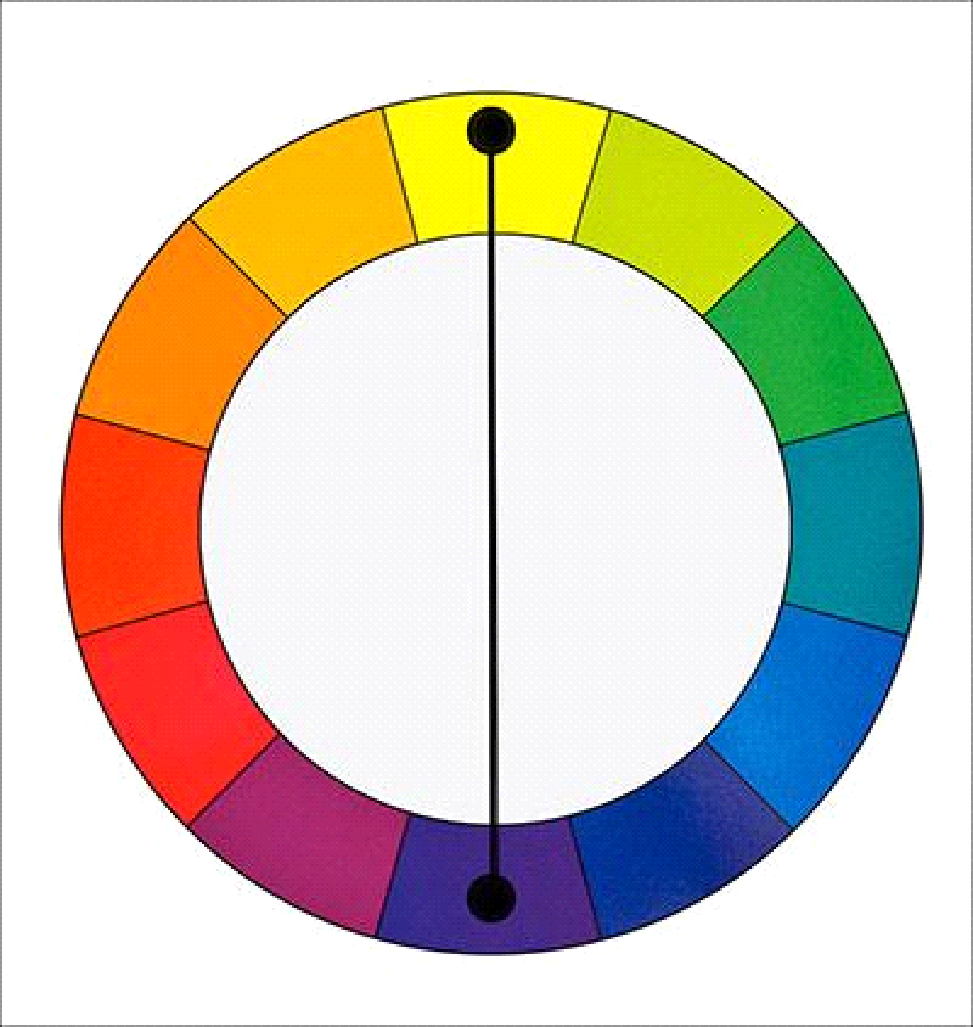
\includegraphics[width=7cm]{imagenes/marcoteorico/disenointeriores/complementario.png}
	\caption{Esquema complementario.\cite{B13}}
	\label{fig:complementario}
\end{figure}

\textbf{Análogo}.- Los colores que se encuentran al lado en el círculo cromático, son agradables juntos. Son la combinación perfecta, ya que son perfectos para cualquier uso, incluso para resaltar y contrastar un elemento específico sin demasiada interrupción. Como regla general, se debe seleccionar un color dominante, un segundo color para sustentar, y un tercer color para acentuar.
\begin{figure}[h!]
	\centering
	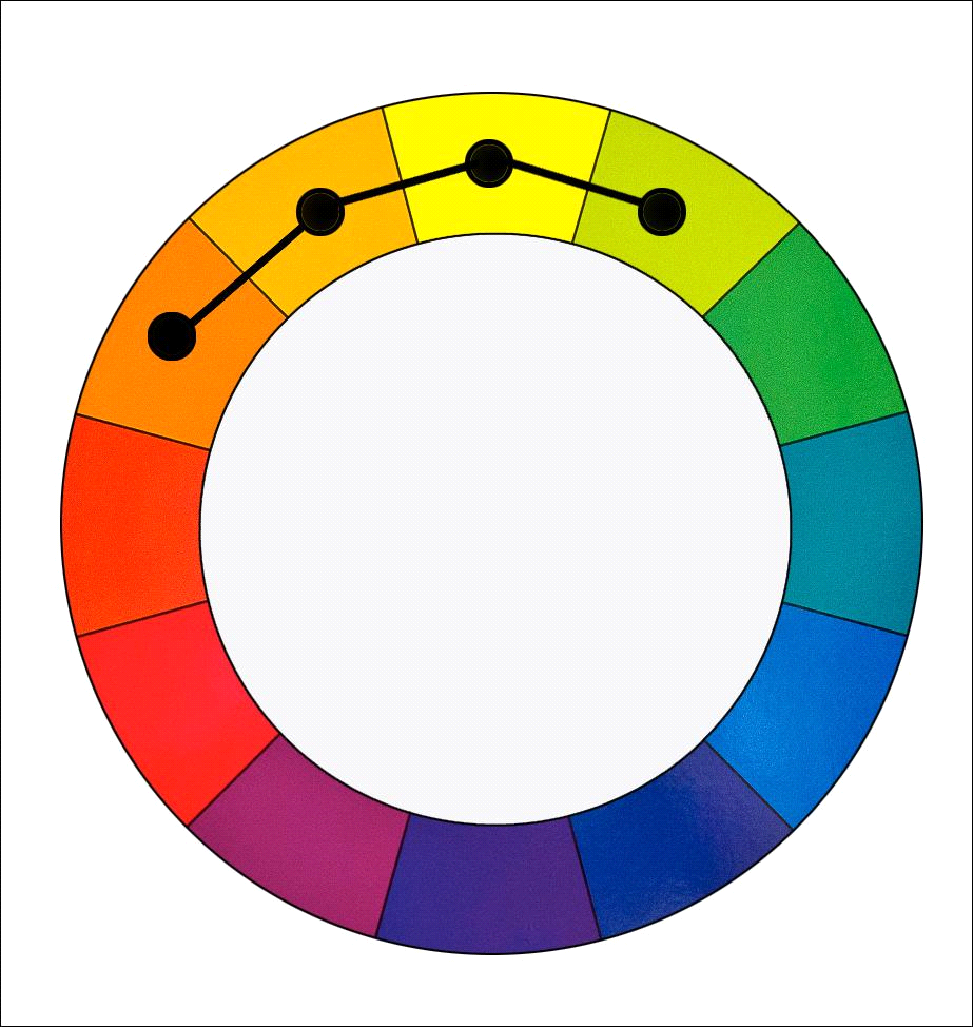
\includegraphics[width=7cm]{imagenes/marcoteorico/disenointeriores/analogo.png}
	\caption{Esquema análogo.\cite{B13}}
	\label{fig:analogo}
\end{figure}


\par 

	   \section{Realidad Aumentada}

\subsection{Definición}
\subsection{Tipos de realidad aumentada}
\subsection{Aplicaciones de la realidad aumentada}
\subsection{Impacto de la realidad aumentada}
\subsection{Plataformas de realidad aumentada para dispositivos mófilves}

\subsubsection{Wikitude}
\subsubsection{ARKit}
\subsubsection{Vuforia}
\subsubsection{ARToolKit}
\subsubsection{ARCore}


----------------------------------------------

La mayoría de las veces asociamos los términos de realidad aumentada con la realidad virtual como si fueran lo mismo, sin embargo existen grandes motivos para detallar sus diferencias de software, hardware y de la interacción con los usuarios. \\.\par 

La realidad aumentada (AR) nos permite sobreponer objetos en tercera dimensión sobre una imagen en tiempo real, obteniendo una mezcla de lo real con lo virtual, mejorando la percepción del mundo real de un usuario. Estas imagenes en tiempo real las podemos obtener con las camaras de smartphones, tablets, smart glasses y computadoras. [1] \\. \par

Por otro lado la realidad virtual (VR) se define como un sistema informático que genera en tiempo real representaciones de una realidad es decir, un mundo virtual donde puede llegar a existir una interacción con el usuario. Muchas de estas simulaciones requieren de gafas de VR compatibles con smartphones o gafas especiales como el Gear VR desarrollado por Samsumg en colaboración con Oculus VR. [2][3] \\. \par

A diferencia de la VR, la AR es una tecnología que complementa  la percepción  e interacción  con el mundo real y permite al usuario estar en un entorno aumentado con información generada por computadora. [1] \\. \par

Actualmente, existen dos grandes representantes en estas tecnologías. Tal vez por criterios de marketing diríamos que Google Glass es el representante de la realidad aumentada, mientras que el Oculus Rift de Facebook sería el representante de la realidad virtual. [4]

	\begin{thebibliography}{X}
	
	\bibitem{B15} \textsc{Hsu, Pei-Hsien}, \textsc{Huang, Sheng-Yang} y \textsc{Lin, Bao-Shuh} ``Smart-Device-Based Augmented Reality (SDAR) Models to Support Interior Design: Rethinking ``Screen” in Augmented Reality", National Chiao Tung University, Taiwan
	
	\bibitem{B01} \textsc{Montes de Oca, Irina} y \textsc{Risco, Lucía},
	``Apuntes de diseño de interiores",
	\textit{Principios básicos de escalas. espacios, colores y más}, primera edicion,
	ECOE EDICIONES
	
	\bibitem{B02} ``FAQ for designers", \textit{Whats is Interior Design}, Interior Design Legislative Coalition of Pennsylvania (IDLCPA), 2011. Recuperado de: https://www.idlcpa.org/forms/resources/FAQforDesigners.pdf
	
	%\bibitem{B26} Kathryn, T.,(2000), feng shui habitación por habitación (12ª ed.). ES, Urano.	
	
	%\bibitem{B24} Harris, C., (2006), dictionary of architecture and construction (4ª ed.). New York, EU, McGraw-Hill.
	
		
	\bibitem{B13} \textsc{Viola, Romina} (11 de mayo de 2016), ``Cómo Elegir la Paleta de Colores", \textit{Parte I: Entender el Color}. Spanish Community Champion | Piktochart. [Online] Recuperado de: https://piktochart.com/es/blog/como-elegir-la-paleta-de-colores-parte-entender-el-color/
	
	
	
	\bibitem{B04} \textsc{Siltanen, Sanni} ``Diminished reality for augmented reality interior design", Springer-Verlag Berlin Heidelberg 2015. Publicado el: 30 de Noviembre de 2015. DOI: 10.1007/s00371-015-1174-z
	DOI 10.1007/978-3-319-54502-8
	
	\bibitem{B05} \textsc{Donggang Yu1, Jesse Sheng Jina},
	``A Useful Visualization Technique: A Literature Review for Augmented Reality and its Application, limitation and future direction", primera edicion,
	School of Design, Communication and Information Technology, The University of Newcastle, Callaghan, NSW 2308, Australia
	
	
	
	\bibitem{B27} \textsc{Furht, Borko} ``Handbook of Augmented Reality",Department of Computer and Electrical Engineering and Computer Science,Florida Atlantic University (),Glades Road 777 33431 Boca Raton, Florida USA,DOI 10.1007/978-1-4614-0064-6
	
	\bibitem{B22} \textsc{Peddie, Jon} ``Augmented Reality Where we will all live", Springer International Publishing AG 2017. Publicado el: 19 de Abril del 2017. DOI 10.1007/978-3-319-54502-8 
	
	\bibitem{B09} \textsc{Monteiro, Paula} and \textsc{Nagele, Aleksandra}, ``Wikitude" \textsc{Company Overview}, Recuperado de: https://s3-eu-west-1.amazonaws.com/wikitude-web-hosting/static-website/2017/07/01728364/Media+page+presentation+-+Wikitude.pdf
	
	
	
	\bibitem{B16} ``Wikitude Products", 29 de agosto de 2018. Recuperado de: https://www.wikitude.com/products/wikitude-sdk/
	
	
	\bibitem{B20} ``ARKit Developer", 2 de Septiembre de 2018. Recuperado de:
	https://developer.apple.com/arkit/
	
	\bibitem{B21} ``ARKit Documentation", 3 de Septiembre de 2018. Recuperado de:
	https://developer.apple.com/documentation/arkit/
	
	
	\bibitem{B12} \textsc{Grahn, Ivar}, ``The Vuforia SDK and Unity3D Game Engine", \textit{Evaluating performanceo on Android Devices}. Linköping University | Department of Computer and Information, Science Bachelor thesis, 16 ECTS, Computer Science 2017, LIU-IDA/LITH-EX-G–17/059–SE
	
	
	\bibitem{B14} ``ARCore Overview", 2 de agosto de 2018. Recuperado de: https://developers.google.com/ar/discover/
	\\
	
	
	%
	
	\bibitem{B03} \textsc{Takahashi, Yoshiyuki} y \textsc{Mizumura, Hiroko},
	``Augmented Reality Based Environment Design Support System for Home Renovation", Toyo  University, Department of Human Environment Design, Faculty of Human Life Design, Oka 48-1, Asaka-shi, Saitama, 351-8510 Japan 
	
	
	
	\bibitem{B06} \textsc{Buerli, Mike} and \textsc{Misslinger, Stefan}, ``Introducing ARKit", \textit{Augmented Reality for iOS. Session 602} Recuperado de: https://devstreaming-cdn.apple.com/videos/wwdc/2017/602pxa6f2vw71ze/602/602
	\_introducing\_arkit\_augmented\_reality\_for\_ios.pdf?dl=1
	
	\bibitem{B07} \textsc{Strandmark, Petter}, ``Augmented reality with the ARToolKit", Recuperado de: http://www.maths.lth.se/matematiklth/personal/petter/rapporter/artoolkit4.pdf
	
	\bibitem{B08} \textsc{Fuster Andújar, Francisco de Asís}, ``Aplicación Android de realidad aumentada para mostrar imágenes históricas de lugares turísticos de interés", Tesis. Escola Tècnica Superior d’Enginyeria Informàtica Universitat Politècnica de València, Valencia, España, 2014.
	
	
	\bibitem{B10} \textsc{Asrul Sani, Nisfu}, ``Google ARCore", Lab Langit 9 - PENS 20-22 de noviembre de 2017. Recuperado de: http://dhoto.lecturer.pens.ac.id/training/arcore/SONI-ARCORE.pdf
	
	\bibitem{B11} \textsc{Kaleda, Yuliya}, ``Add Reality to App with ARCore". Recuperado de: https://downloads.ctfassets.net/2grufn031spf/7AyZDCxxIs0AoOgwOsy0m4/26f89f9d2
	f346dd3c6a55f5d3e2de96e/Yuliya\_Kaleda\_Add\_Reality\_To\_App\_with\_ARCore.pdf
	

	
	
	
	\bibitem{B18} ``OpenGL Documentation". Recuperado el 30 de agosto de 2018 de: https://www.opengl.org/documentation/
	
	\bibitem{B19} ``OpenGL Glut". Recuperado el 30 de agosto de 2018 de: https://www.opengl.org/resources/libraries/glut/spec3/spec3.html
	
    
	
	\bibitem{B23} ``Vuforia Supported-devices". Recuperado el 4 de Septiembre de 2018 de: https://library.vuforia.com/articles/Solution/vuforia-fusion-supported-devices.html
	
	\bibitem{B25} Medina, V. E., (2003). Forma y composición en la arquitectura descontructivista (Tesis doctoral). Escuela Técnica Superior de Arquitectura de Madrid, Madrid, Esp.
	
	\bibitem{B28} ``The new power tool for home improvement". Recuperado el 22 de Octubre de 2018 de: https://canvas.io/
	\bibitem{B29} ``Fingo. Furniture. Try before you buy!". Recuperado el 22 de Octubre de 2018 de: https://itunes.apple.com/us/app/fingo.vybor-mebeli-katalog/id845105741
	\bibitem{B30} ``Electronics -AGILE - Agile Software Technologies". \textit{Mobile -D}. Recuperado el 23 de Octubre de 2018 de: https://itunes.apple.com/us/app/fingo.vybor-mebeli-katalog/id845105741
	
	
\end{thebibliography}

\end{document}


%%%%%%%%%%%%%%%%%%%%%%%%%%%%%%%%%%%%%%%
%%%%%%%    FIN DEL DOCUMENTO    %%%%%%%
%%%%%%%%%%%%%%%%%%%%%%%%%%%%%%%%%%%%%%%
